% =====================================================================================
% Document : rendu du DM2
% Auteur : Xavier Gandibleux
% Année académique : 2018-2019

\section*{Livrable du devoir maison 2 : \\ Métaheuristique GRASP, ReactiveGRASP et extensions}

Les codes sont réalisés sous Julia 0.6.4 en mode mutlicoeur avec la commande : julia -p $<$nombres de coeurs$>$

\vspace{5mm}
\noindent
\fbox{
  \begin{minipage}{0.97 \textwidth}
    \begin{center}
      \vspace{1mm}
        \Large{Présentation succincte de GRASP appliqué sur le SPP}
      \vspace{1mm}
    \end{center}
  \end{minipage}
}
\vspace{2mm}

%\noindent Présenter l'algorithme mis en oeuvre. Illustrer sur un exemple didactique (poursuivre avec l'exemple pris en DM1). Présenter vos choix de mise en oeuvre.

GRASP(Greedy Randomized Adaptative Search Procedure) est un algorithme qui fait un compromis entre
glouton et aléatoire. Contrairement à une descente simple, il ne se limite pas à un optimum local mais explore plusieurs solutions de départ pour des heuristiques d'amélioration. Pour ceci, la construction des solutions de départ sont faites pour avoir de bonnes solutions tout en choisissant de manière aléatoire les variables mises à 1. Ensuite, on relance plusieurs fois les constructions et améliorations pour visiter un plus grand espace de solutions.
Plus précisèment, la construction des solutions se fait de la façon suivante :\\
L'aléatoire dans l'heuristique de construction est controlée par un paramètre $\alpha$.
Ce paramètre limite la qualité des nouvelles variables qui seront choisies pour entrer dans
la solution de départ, les obligeant à dépasser le seuil d'utilité :
\begin{center} $U_{min} + \alpha * (U_{max} - U_{min})$\end{center}
Une variable entrante dépassant ce seuil d'utilité est donc choisie aléatoirement et le processus
se répète jusqu'à ce que la solution de départ ne puisse plus accueillir de nouvelles variables
à 1 sans contredire les contraintes. Ensuite, une heuristique de recherche locale améliore
la solution. Enfin, on compare avec les autres résultats venant des différentes solutions de départ
pour ne garder que la meilleure solution.




La méthode GRASP possède plusieurs avantages par rapport à la méthode de recherche locale et du glouton simple :
\begin{itemize}
\item L'aléatoire permet de tester des solutions initiales différentes (multi-start)
\item Le paramètre $\alpha$ permet de régler la qualité de l'aléatoire et d'ainsi contrôler un peu cet aléatoire, c'est-à-dire d'essayer d'éviter de se laisser la possibilité de sortir d'un optimum local sans non plus choisir une solution de départ de très mauvaise qualité.
\item L'heuristique d'amélioration est lancée sur plusieurs solutions différentes et la meilleure seulement est retenue : cela diminue les chances que cette heuristique se bloque sur un cas particulier de solution initiale.
\end{itemize}


En reprenant l'exemple didactique, pour construire la solution initiale, un $\alpha$ de 0.8 est donnée. Il permet de calculer la limite et de repérer les variables qui ont une utilité au-dessus de celle-ci: le 6,7,4. Au hasard, la 7 est choisie, elle est donc mise à 1 et les autres variables présentes dans les mêmes contraintes que la 7 sont écartées. On répète la même opérations sur les variables restantes, la limite est recalculée et parmi les variables les plus utiles, la 6 est choisie. Ensuite, il ne reste plus que la variable 4 qui est rajoutée à la solution. Il y a ensuite une recherche en profondeur sur cette solution. Dans ce cas, la solution construite est tombée sur la bonne solution donc on ne voit pas d'amélioration. Cette étape est répétée plusieurs fois, pour ne garder que la meilleur solution, puisqu'il est possible selon le choix aléatoire et la limite que l'on ne trouve pas une aussi bonne solution du premier coup.


\vspace{5mm}
\noindent
\fbox{
  \begin{minipage}{0.97 \textwidth}
    \begin{center}
      \vspace{1mm}
        \Large{Présentation succincte de ReactiveGRASP appliqué sur le SPP}
      \vspace{1mm}
    \end{center}
  \end{minipage}
}
\vspace{2mm}

%\noindent Présenter l'algorithme mis en oeuvre. Illustrer sur un exemple didactique (poursuivre avec l'exemple pris en DM1). Présenter vos choix de mise en oeuvre.

Dans le cas d'un Grasp, le choix du paramètre $\alpha$ est complètememt arbitraire.
Pour le choisir plus intelligemment, l'objectif est d'essayer de le régler sur les données en introduisant une phase d'apprentissage durant laquelle on choisira un $\alpha$ qui correspond le mieux possible aux données. Pour ce faire, on choisit de discrétiser
les valeurs possibles de $\alpha$ et de leur attribuer une probabilité égale (loi uniforme).
Après avoir laissé l'algorithme trouver quelques solutions, la probabilité de chaque $\alpha$ est recalculée 
en fonction de la qualité des solutions qu'ils ont engendrés et l'algorithme recommence l'étape précédente afin de trouver d'autres
solutions avec cette nouvelle distribution. Puis, on recommence ce cycle de modifications de probabilités puis de construction et recherche locale de solutions jusqu'à un temps/nombre d'itérations limite. Ainsi,
le paramètre du Grasp apprend et correspond de mieux en mieux aux données sur lesquelles
il est appliqué.


Cette méthode est très intéressante car elle nous permet de ne plus avoir à choisir arbitrairement
le paramètre $\alpha$ mais elle introduit aussi deux autres ``paramètres'' arbitraires :
\begin{itemize}
\item $N_{\alpha}$ : le nombre d'itérations de Grasp avant qu'on ne modifie les probabilités est à première vue arbitraire mais il est possible de discuter du fait de le régler en fonction du nombre de variables.
\item La discrétisation des $\alpha$ : En effet, on discrétise $\alpha$ entre $0$ et $1$ mais on le fait arbitrairement. C'est pourquoi une représentation plus souple se rapprochant d'un $\alpha$ continu pourrait être intéressante à étudier. Pour prendre en compte des valeurs d'$\alpha$ entre $0$ et $1$, il serait possible de choisir aléatoirement un $\alpha$ entre $0$ et $1$ selon des probabilités qui seraient liés à un intervalle de valeurs qui serait réglable selon les qualités des solutions.
  \end{itemize}

En reprenant l'exemple didactique, pour construire la solution initiale, un $\alpha$ est choisi parmi le vecteur d'$\alpha$ résultant de la discrétisation du paramètre. On reprend ensuite la même démarche que dans le GRASP pendant $N_{\alpha}$ itérations. Une fois ce nombre d'itération atteint, si certains $\alpha$ ont contribué à de meilleurs solutions, leurs propabilités d'apparitions sont augmentées. Cette étape est répétée plusieurs fois, ce qui permet de détecter les $\alpha$ les plus efficaces et de les favoriser pour les itérations suivantes. Une fois le critère d'arrêt atteint, on ne garde que la meilleure solution trouvée.

\vspace{5mm}
\noindent
\fbox{
  \begin{minipage}{0.97 \textwidth}
    \begin{center}
      \vspace{1mm}
        \Large{Expérimentation numérique de GRASP}
      \vspace{1mm}
    \end{center}
  \end{minipage}
}
\vspace{2mm}

\begin{example}
  Une éxecution de Grasp sur le Pb 2000rnd0700 avec $\alpha=0.5$
  \begin{figure}[htb!]
    \centering
    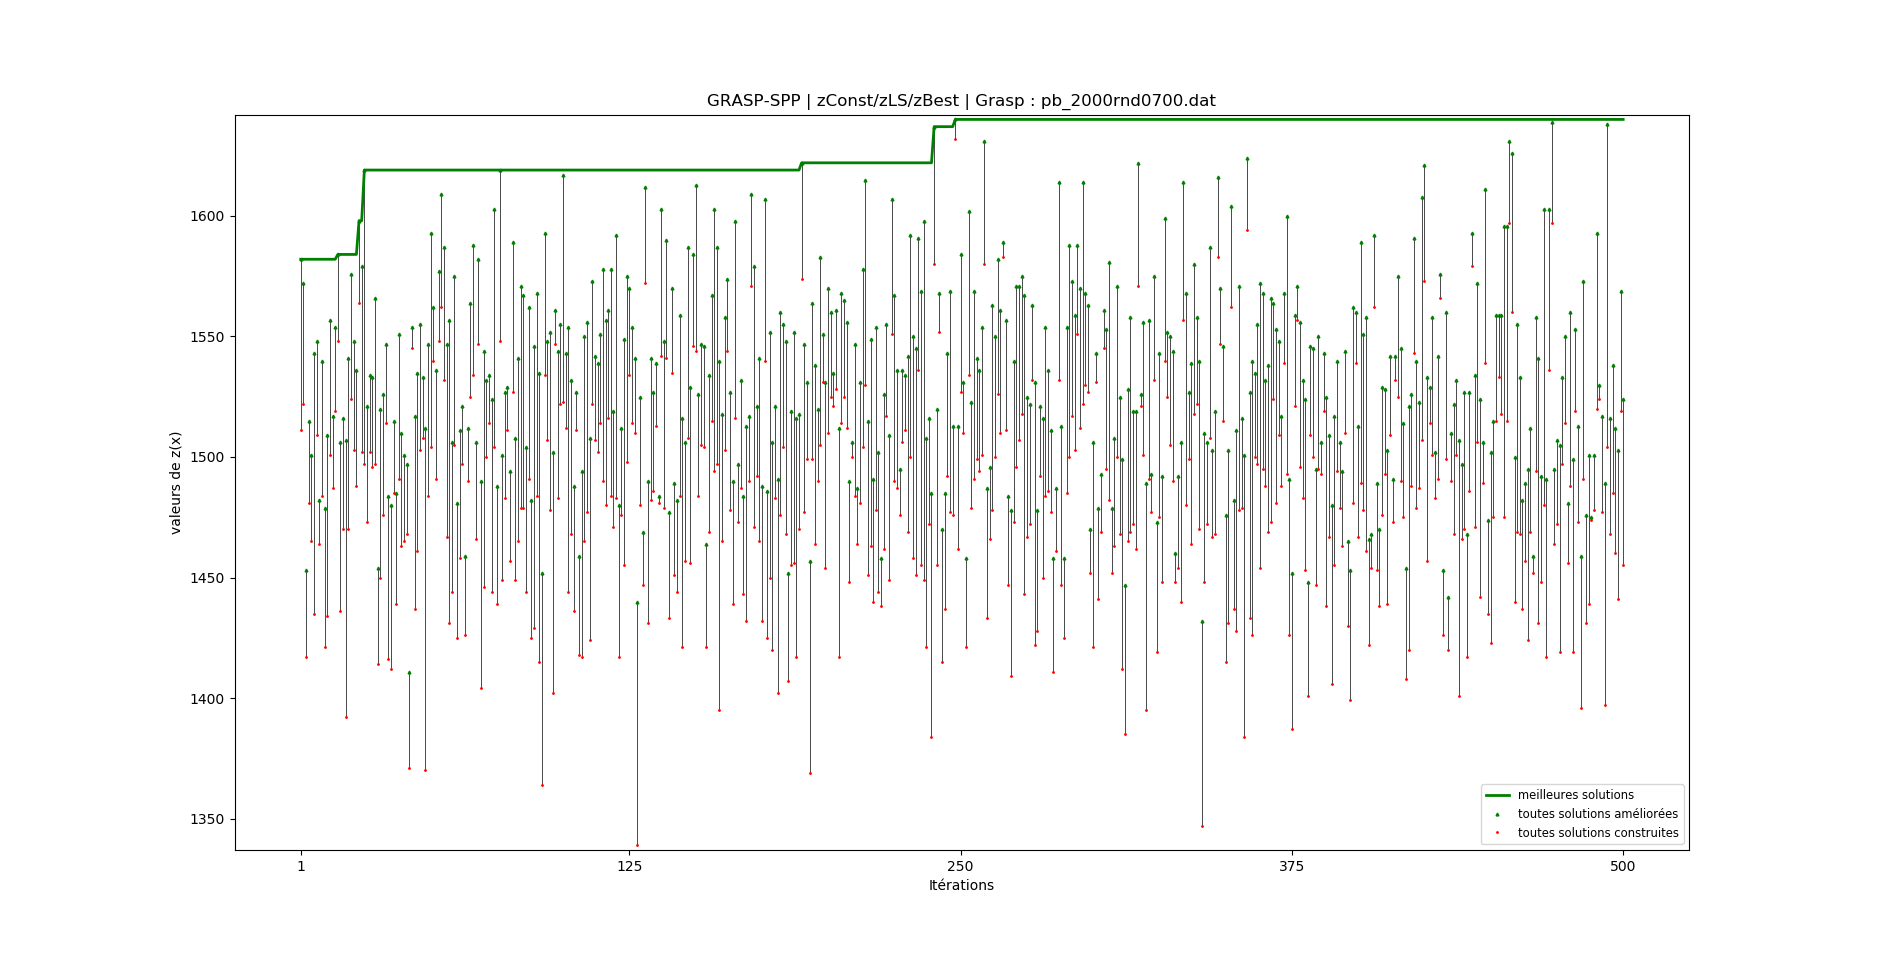
\includegraphics[scale=0.37]{fig/Grasppb2000rnd0700.png}
    %\caption{patate}
    \label{fig:grasp2000rnd0700}
  \end{figure}
\end{example}



Pourcentage de précision de Grasp sur 10 instances pour différents $\alpha$ pendant 10 secondes
\begin{center}
    \begin{tabular}{|c|c|c|c|c|c|c|c|c|c|c|}  
    \hline
    nom de l'instance &  $\alpha=0.2$ &  $\alpha=0.4$ &  $\alpha=0.5$ &  $\alpha=0.6$ & $\alpha=0.7$ &  $\alpha=0.8$ &  $\alpha=0.9$ &  $\alpha=0.95$ \\
     \hline
     pb1000rnd0300 & 76.25 & 82.9 & 83.36 & 86.23 & 86.69 & \textcolor{red}{89.41} & 87.29 & 88.2\\
     \hline
     pb1000rnd0700 & 93.81 & 94.07 & \textcolor{red}{96.24} & 95.18 & 95.13 & 95.04 & 93.63 & 93.01\\
     \hline
     pb100rnd0500 & \textcolor{red}{100} & 100 & 100 & 100 & 99.06 & 98.12 & 98.12 & 98.12\\
     \hline
     pb2000rnd0700 & 78.63 & 88.63 & 88.4 & 88.63 & \textcolor{red}{90.78} & 90.56 & 89.56 & 88.07\\
     \hline
     pb200rnd0100 & \textcolor{red}{99.28} & 98.8 & 97.84 & 100 & 96.88 & 96.88 & 95.91 & 95.19\\
     \hline
     pb200rnd0300 & 96.03 & 96.58 & \textcolor{red}{96.99} & 96.17 & 96.85 & 96.58 & 96.31 & 95.76\\
     \hline
     pb200rnd0700 & 98.9 & \textcolor{red}{99.7} & 99.5 & 98.71 & 98.8 & 98.21 & 97.71 & 96.41\\
     \hline
     pb200rnd0900 & 99.62 & \textcolor{red}{100} & 99.85 & 99.85 & 99.85 & 99.62 & 99.62 & 99.55\\
     \hline 
     pb500rnd0700 & 97.63 & 97.72 & 98.6 & 99.21 & \textcolor{red}{99.74} & 98.69 & 96.67 & 96.67\\
     \hline 
     pb500rnd0900 & 97.54 & 98.75 & 98.88 & 98.66 & 98.93 & \textcolor{red}{98.97} & 98.88 & 98.52\\
     \hline
    \end{tabular}
\end{center}


\paragraph{Remarques : }
\begin{itemize}
\item On observe que le choix du paramètre est important et peut entrainer un écart de précision de plus de 10\%.

\item On remarque aussi que les grandes instances et les instances particulières qui étaient lentes sur les k-p échanges font moins d'itérations de Grasp que les rapides, et donc qu'il est important de régler le $N_{\alpha}$ en conséquence. 
\end{itemize}


\vspace{5mm}
\noindent
\fbox{
  \begin{minipage}{0.97 \textwidth}
    \begin{center}
      \vspace{1mm}
        \Large{Expérimentation numérique de ReactiveGRASP}
      \vspace{1mm}
    \end{center}
  \end{minipage}
}
\vspace{2mm}

%\noindent Présenter le protocole d'expérimentation (env. matériel; budget de calcul; condition(s) d'arrêt).

%\noindent Rapporter graphiquement vos résultats selon $\hat{z}_{min}$, $\hat{z}_{max}$, $\hat{z}_{moy}$ mesurés à intervalles réguliers (exemple de pas de 10 secondes).

%\noindent Rapporter l'apprentissage du paramètre $\alpha$ réalisé par ReactiveGRASP, les valeurs saillantes établies.

%\noindent Présenter sous forme de tableau les résultats finaux obtenus pour les 10 instances sélectionnées.

\begin{example}
  Une éxecution du réactive Grasp sur le Pb 2000rnd0700
  \begin{figure}[htb!]
    \centering
    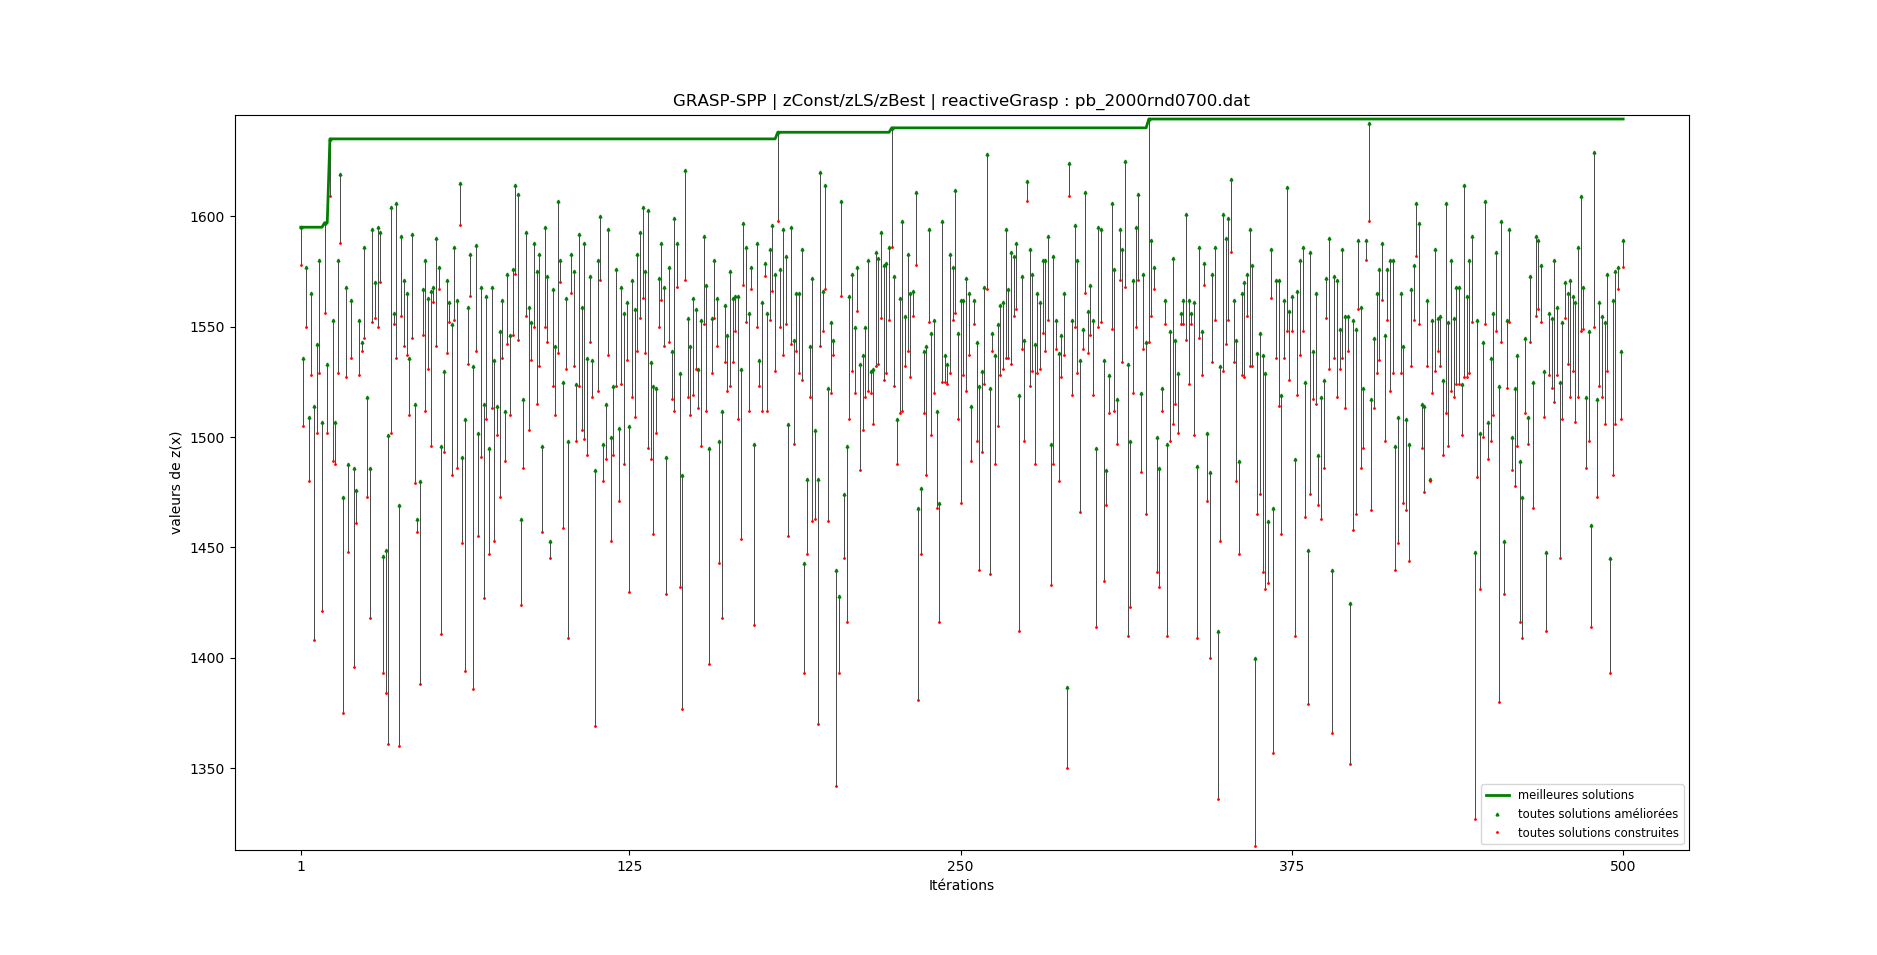
\includegraphics[scale=0.37]{fig/Na=100,nb=500/pb2000rnd0700.png}
    %\caption{patate}
    \label{fig:reactive2000rnd0700}
  \end{figure}

  \vfill
  \break
  
  Distribution finale d'$\alpha$ :
  \begin{figure}[htb!]
    \centering
    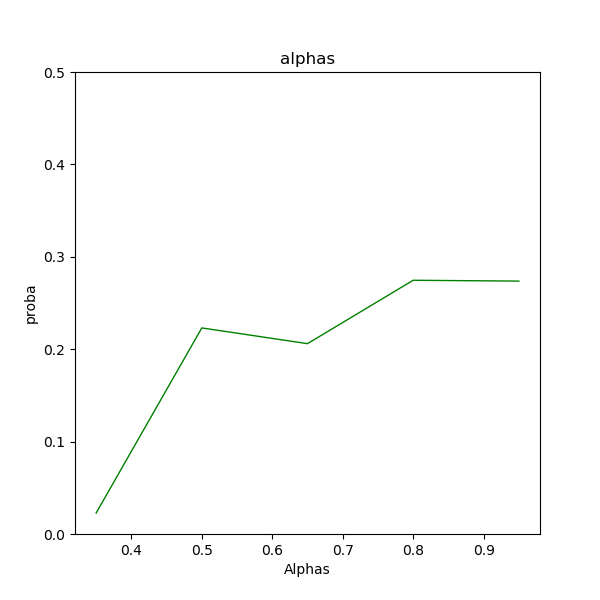
\includegraphics[scale=0.5]{fig/Alpha1.png}
    %\caption{patate}
    \label{fig:alpha1}
  \end{figure}
\end{example}


Pourcentage de précision de Réactive Grasp sur 10 instances pour $\alpha$ dans $[0.35,0.5,0.65,0.8,0.95]$. Avec $N_{\alpha} = 100$ sur 500 itérations.
\begin{center}
    \begin{tabular}{|c|c|c|}  
    \hline
    nom de l'instance & $\alpha$ dominant & précision \\
     \hline
     pb1000rnd0300 & 0.8 & 90.92\% \\
     \hline
     pb1000rnd0700 & 0.65 & 96.19\%\\
     \hline
     pb100rnd0500 & 0.5 & 100\%\\
     \hline
     pb2000rnd0700 & 0.8 & 90.78\%\\
     \hline
     pb200rnd0100 & 0.95 & 98.8\%\\
     \hline
     pb200rnd0300 & 0.95 & 96.31\%\\
     \hline
     pb200rnd0700 & 0.65 & 98.41\%\\
     \hline
     pb200rnd0900 & 0.95 & 100\%\\
     \hline 
     pb500rnd0700 & 0.95 & 98.95\%\\
     \hline 
     pb500rnd0900 & 0.95 & 99.02\%\\
     \hline
    \end{tabular}
\end{center}

% 
alphas : [0.55,0.65,0.75,0.85,0.95]

data/pb_1000rnd0300.dat

alpha dominant : 0.85
accuracy: 93.65%

  data/pb_1000rnd0700.dat

alpha dominant : 0.75
accuracy: 95.71%

  data/pb_100rnd0500.dat

alpha dominant : 0.55
accuracy: 99.84%

  data/pb_2000rnd0700.dat

alpha dominant : 0.85
accuracy: 93.15%

  data/pb_200rnd0100.dat

alpha dominant : 0.95
accuracy: 96.88%

  data/pb_200rnd0300.dat

alpha dominant : 0.95
accuracy: 96.85%

  data/pb_200rnd0700.dat

alpha dominant : 0.65
accuracy: 98.71%

  data/pb_200rnd0900.dat

alpha dominant : 0.95
accuracy: 99.7%

  data/pb_500rnd0700.dat

alpha dominant : 0.85
accuracy: 99.12%

  data/pb_500rnd0900.dat

alpha dominant : 0.85
accuracy: 98.88%



\paragraph{Remarques : }
\begin{itemize}
\item On retrouve sensiblement les mêmes précisions qu'avec les meilleurs Grasp et les $\alpha$ dominants correspondent, sauf sur les instances où le paramètre n'avait pas beaucoup d'influence (par exemple le pb 200rnd0300)
\item On a donc réussi à régler le paramètre $\alpha$ mais au prix d'une discrétisation arbitraire et d'un nouveau paramètre $N_{\alpha}$.
\end{itemize}


\vspace{5mm}
\noindent
\fbox{
  \begin{minipage}{0.97 \textwidth}
    \begin{center}
      \vspace{1mm}
        \Large{Eléments de contribution au bonus}
      \vspace{1mm}
    \end{center}
  \end{minipage}
}
\vspace{2mm}

\paragraph {Path-relinking} \noindent

Le principe du path-relinking\cite{path} est de pousser plus loin les recherches de solutions de bonne qualité à travers l'espace des solutions. Nous partons de solutions trouvées par plusieurs lancés du reactiveGrasp sur une même instance. Nous essayons de partir d'une solution pour rejoindre l'autre en réalisant un swap aléatoire sur les variables qui ont des valeurs différentes dans les deux solutions, tout en restant dans l'espace de solutions admissibles. Sur ce parcours entre les deux, dès qu'une solution trouvée par un swap semble prometteuse (défini arbitrairement), nous réalisons une descente profonde pour rechercher s'il n'y a pas un optimimum, au moins local, plus intéressant.

Observations :  On remarque d'une part, peu d'améliorations sur les petites instance et un path relinking qui boucle sur certaines combinaisons de solutions de départ. Mais d'autre part des améliorations conséquentes (jusqu'à 5\%) sur certaines grosses instances.

Nous avons essayé deux définitions de solution prometteuse, soit on considérait toutes les instances admissibles trouvées prometteuses sans distinction soit on ne prenait que les solutions dont la fonction objectif était supérieur à la solution de départ.

\paragraph {Parallélisme} \noindent


Le parallélisme consiste à envoyer plusieurs parties de nos calculs aux différents coeurs d'une machine et de mutualiser les résultats pour gagner du temps.
Cette méthode se révèle très pratique pour une application du path relinking. On calcule en parallèle deux solutions avec reactive Grasp et on les utilise ensuite pour faire un path relinking.
En julia on utilise la fonction @parallel pour paralléliser les appels de reactive Grasp et la fonciton append! comme réducteur pour concaténer nos solutions dans un vecteur de solutions.

Nous n'avons utilisé le parralélisme seulement pour le path-relinking mais il serait possible de le mettre en oeuvre avec le GRASP et le ReactiveGRASP pour réduire les temps de calculs.

%\noindent \prof{Présenter vos contributions aux aspects proposés en bonus.}



\vspace{5mm}
\noindent
\fbox{
  \begin{minipage}{0.97 \textwidth}
    \begin{center}
      \vspace{1mm}
        \Large{Discussion}
      \vspace{1mm}
    \end{center}
  \end{minipage}
}
\vspace{2mm}


Le problème du Grasp est que son paramètre est arbitraire et peut beaucoup jouer sur la qualité de la solution.
Le Réactive grasp résoud ce problème en apprenant sur les données le $\alpha$ le mieux adapté à celles-ci. Néanmoins, cet apprentissage a besoin d'être réglé aussi et une fois fait, certaines instances restent peu propices à cet apprentissage.
Le path-relinking et le parallélisme permettent d'améliorer les solutions en peu de temps de calculs sur les grandes instances. 


%\noindent \prof{Tirer des conclusions en comparant les résultats collectés avec vos deux variantes de métaheuristiques.}


%\noindent \prof{Quelles sont les recommandations que vous émettez à l'issue de l'étude et avec quelle variante continuez vous l'aventure des métaheuristiques?}


\paragraph{Remarques : }
\begin{itemize}
\item On observe que nos heuristiques sont globalement très mauvaises en temps (par rapport au simplexe) sur les données qui ont des fonctions objectifs uniformes (où toutes les variables ont le même poids)
\item On remarque aussi que la meilleure solution est parfois trouvée par les deux résolutions parallèles. Cela rend le path relinking inutile. On peut en conclure que limiter les grasp par leur nombre d'itérations est plus sécurisant quant à l'efficacité de l'heuristique. Malheureusement, la limite réelle est souvent temporelle.
\end{itemize}

Pour les heuristiques à paramètres, il faut être conscient qu'un bon réglage des paramètres est essentiel pour un bon fonctionnement des heuristiques. Ce réglage peut être fait par l'observation et les tests ou par un apprentissage automatisé. 


\vfill
\break


\bibliographystyle{plain}

\bibliography{xavier}
